% Verification and validation of the axisymmetric (hole-opening) solvers:
% two depth-averaged formulations and two direct free-surface formulations.
%
% Build: see README.md
\documentclass[11pt,a4paper]{article}

\usepackage[margin=2.4cm]{geometry}
\usepackage{amsmath,amssymb}
\usepackage{graphicx}
\usepackage{booktabs}
\usepackage[hidelinks]{hyperref}
\usepackage{caption}
\usepackage{xcolor}

% Slots the campaign has not yet filled. Every one of these is a measurement
% that is scheduled but not made; none is a gap in the argument that the
% measurements already reported establish.
\newcommand{\todo}[1]{\textcolor{red}{\textbf{[to be filled: #1]}}}

\newcommand{\MASS}{\textsf{TC1D-AXI-MASS}}
\newcommand{\ALE}{\textsf{TC1D-AXI-ALE}}
\newcommand{\LAB}{\textsf{AXI-LAB}}
\newcommand{\COM}{\textsf{AXI-COMOVING}}
\newcommand{\Ohsb}{\mathrm{Oh}}
\newcommand{\Vtc}{V_{TC}}

\title{Verification and validation of axisymmetric solvers for
hole opening in a viscous sheet}
\author{%
  Vatsal Sanjay\thanks{%
    \href{mailto:vatsal.sanjay@comphy-lab.org}{vatsal.sanjay@comphy-lab.org};
    ORCID \href{https://orcid.org/0000-0002-4293-6099}{0000-0002-4293-6099}.}\\[2pt]
  \normalsize CoMPhy Lab, Department of Physics, Durham University,\\
  \normalsize Science Laboratories, South Road, Durham DH1 3LE, United Kingdom}
\date{\today}

\begin{document}
\maketitle

\begin{abstract}
We document four solvers for the axisymmetric Taylor--Culick problem --- the
opening of a circular hole in a viscous sheet --- and the evidence that each
solves the equations it claims to. Two are depth-averaged: a Lagrangian
per-radian mass coordinate carrying the radial metric as an unknown, and an
arbitrary Lagrangian--Eulerian (ALE) solver in the physical radius. Two resolve
the free surface directly: a laboratory-frame calculation on a graded annulus,
and a co-moving window that translates outward with the rim. The depth-averaged
equations were derived independently and agree term for term with Savva \&
Bush's (3.15)--(3.16); the direct formulations were audited line by line against
two independent implementations of the axisymmetric operators. In this geometry
a radial translation is not a Galilean boost, so the co-moving trick that serves
the planar sheet has no analogue: the laboratory frame is limited by the finite
sheet it must mesh, and the window formulation, not a change of variables, is
what represents a semi-infinite sheet. Verification is by an internal-check
ladder, whose gate is the planar limit: at large initial radius $R_{0}$ both
depth-averaged solvers reproduce the validated planar solver with a deviation
falling as $0.37/R_{0}$, under the $2/R_{0}$ admission bound at every rung, and
the direct solver reproduces the validated planar retraction speed to $0.13\%$
at $R_{0}=100$. Against the 2024 volume-of-fluid campaign the direct solver
agrees to $1.6\%$ in radius and $1.8\%$ in speed, systematically and at face
value. The depth-averaged model at $R_{0}=1$ does not reproduce the direct
solution: the two available tip closures bracket it from above and below,
$0.9966$ and $0.8976$ against $0.9613$ at $t^{*}=100$, which locates the
discrepancy in the edge condition rather than in the bulk. Four numerical traps
found in the course of this work are recorded with the evidence that identified
each, because three of them return a plausible wrong answer or a misleading
failure rather than an error.
\end{abstract}

\section{Scope}
\label{sec:scope}

This note covers the Newtonian axisymmetric strand: four solvers, the checks
each passes, and the small number of end-to-end comparisons made against
external data. It is a companion to the planar validation note, and it inherits
that note's conventions, its planar solvers as references, and its warning
about Ohnesorge conventions.

Two limits on what follows should be stated at the outset rather than
discovered in \S\ref{sec:validation}. First, the comparisons in
\S\ref{sec:validation} are one end-to-end run per question. This strand exists
to establish that the axisymmetric machinery is correct and that its answers
are not obviously wrong, not to benchmark it exhaustively; a sweep in
$\Ohsb$ and $R_{0}$ is deliberately out of scope. Second, the internal checks
of \S\ref{sec:verification} test discretisations against the equations and
against each other. They are not evidence that the depth-averaged model
describes a real opening hole, and \S\ref{sec:validation} shows a case in which
it plainly does not.

\subsection{Nomenclature and units}

The non-dimensionalisation is unchanged from the planar work: $\rho = \sigma =
h_{0} = 1$ with $h_{0}$ the \emph{full} sheet thickness, so the half-thickness
is $1/2$ and the Taylor--Culick speed \cite{taylor1959,culick1960} is
$\Vtc = \sqrt{2\sigma/\rho h_{0}} = \sqrt{2}$. Throughout, $\Ohsb =
\mu/\sqrt{2 h_{0}\rho\gamma}$ is the Savva \& Bush Ohnesorge number
\cite{savva2009}, the coded viscosity is $\mu = \sqrt{2}\,\Ohsb$, the viscous
clock is $\tau_{\mathrm{vis}} = \mu/2$ and $t^{*} = t/\tau_{\mathrm{vis}}$. The
reported speed is $u^{*} = \dot{R}/\Vtc$, which tends to unity.

One parameter is new: the initial hole radius $R_{0}$, in units of $h_{0}$.
The combination that governs the early behaviour is
$R_{0}^{*} = R_{0}/(\Ohsb\,h_{0})$, the Savva \& Bush similarity variable
\cite{savva2009}; $R_{0}^{*}\ll 1$ is the small-hole regime in which the hole
grows exponentially and $R_{0}^{*}\gg 1$ is the regime that starts like the
planar sheet. It is worth computing before choosing a test, because neither
closed form is a clean target in between.

All four are built on the same symbolic finite-element framework
\cite{diddens2023}, which derives residuals and Jacobians from the weak forms
written below. Their entry points; all four modules live in
\texttt{simulationCases/}:

\begin{center}
\footnotesize
\begin{tabular}{@{}llp{0.46\textwidth}@{}}
\toprule
name & module & what it is \\
\midrule
\MASS & \texttt{trouton1d\_axi.py}
  & depth-averaged, per-radian Lagrangian mass coordinate, fixed domain,
    radial metric carried as an unknown \\
\ALE & \texttt{trouton1d\_ale\_axi.py}
  & depth-averaged, physical radius on a moving mesh \\
\LAB & \texttt{axisymmetric\_lab.py}
  & free-surface Navier--Stokes, laboratory frame, graded annulus \\
\COM & \texttt{axisymmetric\_comoving.py}
  & free-surface Navier--Stokes, window of fixed length translating with the
    rim \\
\bottomrule
\end{tabular}
\end{center}

\section{The depth-averaged axisymmetric model}
\label{sec:model}

The guiding choice is a \emph{metric} formulation. The grids stay
one-dimensional exactly as in the planar codes; axisymmetry enters through the
$r$-weighted measure and the hoop terms of the governing equations, and not
through a second spatial dimension. Everything below was re-derived from first
principles and then checked term by term against Savva \& Bush's equations
\cite{savva2009}; the planar limit reproduces the residuals of the planar
modules exactly, which is what the check of \S\ref{sec:planarlimit} measures.

\subsection{Membrane form}

Let $r$ be the radial coordinate, $R(t)$ the hole edge, and let the film occupy
$r > R$. With $u(r,t)$ the depth-averaged radial velocity and $h(r,t)$ the full
thickness, the plane-stress ($\sigma_{zz}=0$) viscous membrane stresses, with the
extensional response of Trouton \cite{trouton1906}, are
%
\begin{equation}
  \sigma_{rr} = 2\mu\left(2 u_{r} + \frac{u}{r}\right),
  \qquad
  \sigma_{\theta\theta} = 2\mu\left(u_{r} + 2\frac{u}{r}\right),
  \qquad
  N_{rr} = h\sigma_{rr}, \quad N_{\theta\theta} = h\sigma_{\theta\theta},
  \label{eq:membrane}
\end{equation}
%
and the depth-averaged mass and momentum balances are
%
\begin{align}
  \frac{\partial h}{\partial t}
    + \frac{1}{r}\frac{\partial}{\partial r}\left(r u h\right) &= 0,
  \label{eq:axi-mass}\\[2pt]
  h\left(\frac{\partial u}{\partial t} + u\frac{\partial u}{\partial r}\right)
    &= \frac{\partial N_{rr}}{\partial r}
       + \frac{N_{rr}-N_{\theta\theta}}{r} .
  \label{eq:axi-mom}
\end{align}
%
Equation \eqref{eq:axi-mass} is Savva \& Bush's (3.15). Expanding the
right-hand side of \eqref{eq:axi-mom} gives
%
\begin{equation}
  4\nu h\left(u_{rr} + \frac{u_{r}}{r} - \frac{u}{r^{2}}\right)
  + 2\nu h_{r}\left(2u_{r} + \frac{u}{r}\right),
  \label{eq:axi-expanded}
\end{equation}
%
which is their (3.16) multiplied through by $h$; the identity was verified by
expanding their form
$(4\nu/h)\left[\left((h/r)(ur)_{r}\right)_{r} - u h_{r}/(2r)\right]$ and
matching term for term. Two terms are new relative to the planar model: the
metric weight in the mass flux and in the stress divergence, and the hoop stress
$N_{\theta\theta}/r$. Both vanish as $h_{0}/R \to 0$, so the planar operator is
the exact $R_{0}\to\infty$ limit --- which is a statement the code can be made
to prove, and \S\ref{sec:planarlimit} does.

The distributed capillary term of Savva \& Bush's (3.16) stays \emph{off} by
default, exactly as in the planar solvers: the tip closure below already
carries the capillary driving, so a bulk curvature term would double-count it.
For a cell-constant thickness the elementwise gradient of $h$ is identically
zero, so switching bulk capillarity on is not a flag but a change of variable
--- it would have to arrive together with $f = h^{2}$, whose curvature is the
only form bounded at the tip \cite{savva2009}. The solver rejects the
combination rather than integrating a silently vanishing term.

\subsection{Mass-coordinate form, and the metric field $w = r^{2}/2$}
\label{sec:mass}

With the per-radian mass coordinate $\mathrm{d}m = r h\,\mathrm{d}r$ the tip
sits at $m=0$ and the domain $[0,M]$ is fixed, which is the property that makes
this the accurate late-time formulation. The price is that
$\partial_{r} = r h\,\partial_{m}$ carries the radius, so the radial map appears
in every residual and must be carried as an unknown.

The choice made here is to carry $w = r^{2}/2$ on continuous piecewise-linear
elements rather than $r$ itself, constrained by
%
\begin{equation}
  \frac{\partial w}{\partial m} = \frac{1}{h},
  \qquad r = \sqrt{2w},
  \label{eq:metric}
\end{equation}
%
together with one global scalar $R(t)$ satisfying $\dot{R} = u|_{m=0}$ and
$w|_{m=0} = R^{2}/2$. Three properties recommend \eqref{eq:metric} over the
obvious alternatives. It is \emph{linear} in the carried unknown, where
$r_{m} = 1/(rh)$ is not. With $w$ piecewise linear and $h$ cell-constant both
sides are cell-constant, so \eqref{eq:metric} is a per-cell statement and the
discrete radial map is exactly consistent with the discrete mass distribution,
cell by cell, to round-off --- a property that is measured rather than assumed
(\S\ref{sec:verif-mass}). And $r^{2} = 2w$ exactly, so every even power of the
radius in the residuals is a polynomial in the unknown and only the odd powers
cost a square root. Evolving $r_{t} = u$ pointwise instead is consistent only in
the continuum: it lets the discrete radial map drift away from the discrete mass
it is meant to describe.

The momentum weak form is written so that the only reciprocal anywhere in the
residual is a single guarded $1/r^{2}$. With test function $v$ and a Cartesian
measure in $m$,
%
\begin{equation}
  \int u_{t}v\,\mathrm{d}m
  + \int\left[4\mu r^{2}h^{2}u_{m} + 2\mu h u\right]v_{m}\,\mathrm{d}m
  + \int\left[2\mu h u_{m} + \frac{4\mu u}{r^{2}}\right]v\,\mathrm{d}m
  - 2R\,v(0) = 0 .
  \label{eq:massweak}
\end{equation}
%
Coding the hoop term literally as $\sigma_{\theta\theta}/r$ instead introduces a
spurious $1/r$ that cancels analytically but not numerically. That is the
restructuring a future refactor is most likely to reintroduce, and it is why
the dissipation check of \S\ref{sec:verif-mass} exists: setting $v = u$
collapses the viscous terms to
$\int 4\mu\left[u_{r}^{2} + u_{r}(u/r) + (u/r)^{2}\right]\mathrm{d}m$, a
positive-definite form with eigenvalues $1/2$ and $3/2$, so a sign error in the
hoop term drives it negative immediately.

Discretisation follows the planar production choice: $h$ cell-constant, $u$ and
$w$ continuous piecewise linear, no midside velocity degrees of freedom
anywhere, BDF2 in time. This is the finite-element realisation of the staggered
arrangement Savva \& Bush adopt, following Eggers \& Dupont
\cite{eggers1994}, for the same reason: they report that a non-staggered grid
introduced spurious oscillations in the curvature at long times
\cite{savva2009}. The co-located quadratic arrangement is retained in the
planar module for reproducing older runs and is deliberately unavailable here,
because it is non-convergent.

\subsection{ALE form}
\label{sec:aleform}

\ALE\ integrates \eqref{eq:axi-mass}--\eqref{eq:axi-mom} in the physical radius
on $[R(t), R_{\mathrm{out}}]$, with the mesh moving under a Laplace-smoothed
mesh equation. In one dimension that smoothing is the affine stretch
$x(X) = R(t) + \left(R_{0}+\ell_{0}-R(t)\right)(X-R_{0})/\ell_{0}$, which is
precisely the mapping Savva \& Bush use \cite{savva2009}, applied to the offset
domain.

Here the measure does the work. Selecting the axisymmetric coordinate system
attaches the factor $2\pi r$ to \emph{every} integral the framework assembles on
the domain, including the zero-dimensional point contribution a boundary
condition makes at a mesh endpoint. Integrating \eqref{eq:axi-mom} by parts
under that measure leaves the full $N_{rr}$, including its $u/r$ part, in the
flux slot, and the hoop term outside it as
%
\begin{equation}
  \underbrace{\int N_{rr}\,v_{r}\,(2\pi r)\,\mathrm{d}r}_{\text{flux slot}}
  \qquad\text{and}\qquad
  \underbrace{\int \frac{N_{\theta\theta}}{r}\,v\,(2\pi r)\,\mathrm{d}r
    = \int N_{\theta\theta}\,v\,(2\pi)\,\mathrm{d}r}_{\text{hoop term}} .
  \label{eq:aleweak}
\end{equation}
%
The $1/r$ written explicitly in the hoop term is therefore not a numerical
convenience; it is exactly what cancels the extra radius the measure would
otherwise leave on that term. This form was verified by expansion rather than
assumed, because it is the one place where the automatic measure and the
hand-written residual have to agree.

Both fields are continuous piecewise linear here. The mass equation carries an
advective term in this frame, so a cell-constant thickness would need an upwind
flux; co-location is safe because the parasitic mode that rules it out in the
planar mass-coordinate solver lives on midside nodes, which a linear line mesh
does not have.

One property of the affine map is a known limitation rather than a defect. It
compresses resolution uniformly across the domain as $R$ grows, so it loses
near-tip resolution by orders of magnitude if $R$ itself grows by orders of
magnitude --- which is the small-hole exponential regime. An area- or
arclength-preserving stretch is the recorded upgrade path.

\subsection{Tip closure, and an optional geometric correction}
\label{sec:tip}

At leading order the closure is unchanged from the planar case: the massless-cap
force balance $N_{rr}(R) = -2\gamma_{\text{total}} = -2$. Savva \& Bush's
axisymmetric jump condition (3.20) is the same $[u_{r}] = -1/4$ as their planar
(2.22), so the constant is the planar one. What the geometry adds is supplied by
the measure: under an $r$-weighted measure the boundary term automatically
carries the factor $r_{\mathrm{tip}} = R$, giving the correct per-radian pull
$2\gamma R$. In the mass-coordinate solver this makes the boundary value
nonlinear in a global unknown, which the symbolic Jacobian handles without
special-casing.

The first geometric correction is available behind a flag and is off by default.
The toroidal rim surface opposes opening with a force $\gamma\pi
h_{\mathrm{tip}}/(2R)$ per unit edge length, so
%
\begin{equation}
  N_{rr}(R) = -2 + \frac{\pi h_{\mathrm{tip}}}{2R} .
  \label{eq:tipcorr}
\end{equation}
%
It was derived two ways --- as the surface-energy release rate of the cap, and
by integrating the azimuthal Laplace pressure $\gamma/R$ over the cap arc
$\pi h_{\mathrm{tip}}/2$ --- and it is the $O(h/R)$ effect that the early-time
analysis of Savva \& Bush neglects, their scaling requiring $h_{0}/R_{0}\ll1$.
At $R_{0} = h_{0} = 1$ that correction is $O(1)$ at $t=0$. The flag therefore
exists to \emph{measure} the term's importance against a direct calculation, not
to assert that it belongs in the leading-order model;
\S\ref{sec:bracket} is that measurement.

\subsection{Why $R_{0}=0$ is excluded}

A vanishing initial hole is excluded on four independent grounds, and it is
worth recording all four because any one of them alone reads as a numerical
inconvenience. The early similarity solution $R(t) = R_{0}\exp(t/2\tau_{\mathrm{vis}})$
is linear in $R_{0}$, so a zero hole never opens. The mass map degenerates,
$\mathrm{d}r/\mathrm{d}m\to\infty$. The edge force and the rim mass both vanish,
leaving the tip acceleration a $0/0$. And the azimuthal curvature $1/R$
diverges: below the Taylor \& Michael threshold at $R\sim h_{0}$ a hole closes
rather than opens \cite{taylor1973}. Production depth-averaged runs use
$R_{0}\ge 5$, which is Savva \& Bush's own smallest; $R_{0}\sim1$ sits at about
twice the closing threshold and is reserved for the comparison of
\S\ref{sec:bracket}, where it is the direct solver's initial condition that
forces the choice.

\section{Two direct formulations, and the frame question}
\label{sec:dns}

\subsection{The laboratory frame on a graded annulus}

\LAB\ solves the incompressible Navier--Stokes equations in the liquid only,
with a true free surface, on an annular domain $r\in[R(t), R_{\mathrm{out}}]$
with the midplane $z=0$ a symmetry line. The hole behind the rim is not meshed,
so the liquid domain \emph{shrinks} as the hole opens. The mesh is graded to the
current tip and coarsens to the quiescent far film, which needs only about two
elements across the half thickness.

The axisymmetric coordinate system is already the metric formulation: the mesh
stays two-dimensional in $(r,z)$, the measure gains $2\pi r$, the operators gain
their hoop terms, and the free-surface condition in surface-divergence form
carries \emph{both} principal curvatures with no curvature code written
anywhere. That last point is the one worth checking rather than trusting, and
the static-droplet discriminator of \S\ref{sec:verif-lab} checks it.

The initial geometry is the annular translate of the planar one: tip at
$(R_{0},0)$, a cap semicircle of radius $1/2$ centred at $(R_{0}+1/2,0)$, and
the film running out to $R_{\mathrm{out}}$. At $R_{0}=1$ this matches the
initial condition of the 2024 volume-of-fluid campaign \cite{basilisk} exactly, which is what
makes the comparison of \S\ref{sec:basilisk} like for like. The hole radius
$R(t)$ is a pure observable --- the minimum radial mesh coordinate on the free
surface --- and $\dot{R}$ follows by differentiation. Because no fluid crosses
any boundary, exact global volume conservation is available free as a sharp
correctness diagnostic, and it is monitored on every output.

\subsection{A radial translation is not a Galilean boost}
\label{sec:frame}

In the planar problem the retraction can be computed in a frame that follows the
rim: freeze the tip, blow the far film in at $-U$, promote $U$ to a global
degree of freedom. That trick has no axisymmetric analogue. A radial
translation of an axisymmetric geometry is not a Galilean boost, so there is no
change of variables in which the far film is uniformly in motion and the
governing equations are unaltered. Two consequences follow, and both are
structural rather than matters of taste.

First, \LAB\ carries no global frame-velocity unknown, no bulk force for frame
acceleration, and no tip-pinning constraint --- because none of that machinery
exists, none of the framework's recorded traps can fire in it. Second, the fixed
outer wall at $R_{\mathrm{out}}$ must contain the whole trajectory, so the
reachable end time is bounded by the mesh budget rather than by the physics.
That is the honest limitation of the laboratory frame, and it is the reason for
the second direct solver.

\subsection{The co-moving window}
\label{sec:comoving}

\COM\ keeps the \emph{window length} $L$ fixed and drags it outward with the
rim, so the degree-of-freedom count is independent of the end time. This is an
ALE window translation, not a change of variables: the coordinate system remains
axisymmetric, the mesh coordinates carry the true radius, and the velocities are
laboratory-frame throughout. It is the proper semi-infinite-sheet formulation of
this problem, and it is not equivalent to any co-moving frame.

Three consequences are worth stating. There is no non-inertial correction, and
porting the planar one would be a physics error, not a conservative choice. The
far boundary is a genuine inflow of quiescent liquid. And volume is
\emph{not} conserved, so the free diagnostic of the laboratory case is replaced
by an exact modified identity: the volume at time $t$ must equal the initial
volume plus the liquid the advancing far edge has swept in,
$V(t) = V(0) + \tfrac{\pi}{2}\left[(X+L)^{2}-(X_{0}+L)^{2}\right]$ for a film of
half-thickness $1/2$, with $X$ the window position. That identity is checked at
every output.

The retraction speed here is a solved unknown rather than a post-processed
difference. A second global degree of freedom $U$ satisfies $\dot{X} - U = 0$
and is differentiated by the same BDF2 scheme as everything else, instead of by
a first-order difference across a geometrically stretching output schedule. The
driver logs both, and their difference is a free accuracy monitor on the output
cadence.

\section{Verification}
\label{sec:verification}

Each solver carries a check suite that runs it through the same driver the
campaign uses, so the checks exercise the production path rather than a bespoke
harness. The suites are

\begin{center}
\small
\begin{tabular}{@{}ll@{}}
\toprule
solver & check suite \\
\midrule
\MASS & \texttt{validation/trouton1d\_axi\_checks.py} \\
\ALE  & \texttt{validation/trouton1d\_ale\_axi\_checks.py} \\
\LAB  & \texttt{validation/axi\_smoketests.py} \\
\bottomrule
\end{tabular}
\end{center}

The ordering within a suite is chosen for cost, not for logic. The gate is the
planar limit: it is the only check that compares against an independently
validated solver rather than against the formulation's own internal structure,
and until it passes nothing else in the suite is evidence of correctness. A
metric constraint can be satisfied exactly by a wrong metric, and a
positive-definite dissipation stays positive under a wrong prefactor.

\subsection{The mass-coordinate solver}
\label{sec:verif-mass}

\emph{Metric consistency.} The per-cell residual of \eqref{eq:metric} is
$|w_{m}-1/h| = 5.8\times10^{-14}$ at worst over all cells and all outputs. This
is the structural payoff of the staggering, and if it ever drifts the
discretisation of $w$ is wrong.

\emph{Metric closure.} The global identity
$r(M)^{2} = R^{2} + 2\int_{0}^{M}\mathrm{d}m/h$ holds to
$7.5\times10^{-16}$ relative. Mass itself is exact by construction in this
coordinate, since $M$ does not move; the metric identity is what stands in its
place.

\emph{Tip-thickness identity.} The closure implies exactly
$\mathrm{d}h_{\mathrm{tip}}/\mathrm{d}t = 1/(2\mu) -
h_{\mathrm{tip}}u_{\mathrm{tip}}/(2r_{\mathrm{tip}})$. Integrating that ordinary
differential equation alongside the run, using the solver's own
$u_{\mathrm{tip}}$ and $r_{\mathrm{tip}}$, the solver's first-cell thickness
matches it to $6.7\times10^{-4}$ relative. The planar limit of the same identity
recovers $h_{\mathrm{tip}} = 1 + t^{*}/4$; its late-time axisymmetric limit is
$h_{\mathrm{tip}}\to t^{*}/6$, azimuthal stretching thinning the rim by exactly
$2/3$ relative to planar. That last result was derived independently twice and
is the headline non-planar prediction of the reduced model.

\emph{Early exponential growth.} In the small-hole regime, at $\Ohsb = 100$ and
$R_{0}=5$ so that $R_{0}^{*}=0.05\ll1$, the fitted logarithmic growth rate of
$R(t)$ is within $1.04\%$ of $1/(2\tau_{\mathrm{vis}})$, which is Savva \&
Bush's (3.30). The check reports the rate over four fit windows rather than one,
so the sensitivity to that choice is visible rather than hidden inside a pass.
The similarity solution is an early-time law that an impulsive start has to
settle onto, so the first fraction of a viscous time is a start-up transient
with a rate below the asymptote, and the window has to be chosen to exclude it.

\emph{Dissipation.} The depth-averaged dissipation density is non-negative at
every cell and every output, and finite everywhere. Alongside it the discrete
energy budget $\mathrm{d}(\mathrm{KE})/\mathrm{d}t = 2Ru_{\mathrm{tip}} - D$ is
reported, with a worst relative residual of $5.1\times10^{-3}$; that number is
limited by the finite-difference time derivative taken on a geometric output
cadence, not by the balance, and it is reported rather than gated for that
reason.

\subsection{The ALE solver}
\label{sec:verif-ale}

\emph{Mass conservation.} The relative drift of $2\pi\int h r\,\mathrm{d}r$ is
$5.8\times10^{-9}$ at $2000$ elements. The drift is spatial-error dominated:
doubling the number of timesteps at fixed mesh does not move it, whereas the
mesh ladder gives $3.6\times10^{-8}$, $9.1\times10^{-9}$ and
$5.8\times10^{-9}$ at $800$, $1600$ and $2000$ elements.

\emph{Mesh affinity.} The mesh sits on the affine stretch of
\S\ref{sec:aleform} to $\sim10^{-14}$ of the domain length, so the mesh-motion
solution is verified rather than assumed.

\emph{Early exponential growth.} As above, within $3\%$ of $1/\mu$ over
$t^{*}\le2$ at $\Ohsb=100$, $R_{0}=5$ ($R_{0}^{*}=0.035$). The window is
justified by where the regime ends: the exponential law breaks down once $R$
approaches $\Ohsb\,h_{0}$, here at $t^{*}\approx6$, and $R(t^{*}=2)\approx13.6$
is comfortably inside it.

\emph{Cross-solver.} At $\Ohsb=1$, $R_{0}=5$, the two depth-averaged solvers
agree to $\max|\Delta u^{*}| = 7.3\times10^{-6}$. They share the equations and
nothing else: a Lagrangian mass coordinate with a carried metric against a
physical radius on a moving mesh, a cell-constant thickness against a continuous
one, a nonlinear-in-$R$ boundary value against a measure-supplied one. That
agreement is the strongest internal evidence available for either of them.

\subsection{The planar limit, which is the gate}
\label{sec:planarlimit}

Both depth-averaged solvers are compared against the validated planar solver at
matched $\Ohsb$, matched end time, matched timestep and matched output
schedule, so the comparison is row by row with no interpolation. The meshes are
matched by \emph{tip cell in radius} and not by element count: the axisymmetric
domain is a mass, so an equal element count would place a systematically
different cell at the tip and contaminate the difference with a discretisation
offset that does not scale with $1/R_{0}$.

\begin{center}
\small
\begin{tabular}{@{}lccccc@{}}
\toprule
$R_{0}$ & 50 & 100 & 200 & 400 \\
\midrule
\MASS, $\max|\Delta u^{*}|$ & $3.355\times10^{-3}$ & $2.717\times10^{-3}$
  & $1.675\times10^{-3}$ & $9.246\times10^{-4}$ \\
\MASS, $R_{0}\max|\Delta u^{*}|$ & $0.168$ & $0.272$ & $0.335$ & $0.370$ \\
\ALE,\ $\max|\Delta u^{*}|$ & $3.357\times10^{-3}$ & $2.718\times10^{-3}$
  & $1.675\times10^{-3}$ & --- \\
\ALE,\ $R_{0}\max|\Delta u^{*}|$ & $0.168$ & $0.272$ & $0.335$ & --- \\
bound $2/R_{0}$ & $4.0\times10^{-2}$ & $2.0\times10^{-2}$
  & $1.0\times10^{-2}$ & $5.0\times10^{-3}$ \\
\bottomrule
\end{tabular}
\end{center}

Every rung is inside the $2/R_{0}$ bound with an order of magnitude to spare,
and the scaled deviation $R_{0}\max|\Delta u^{*}|$ rises towards a constant
$0.37\pm0.03$ rather than towards zero or towards infinity, which is the
statement that the leading correction is $O(1/R_{0})$. The observed order in
$1/R_{0}$ improves down the ladder, $0.30$, $0.70$, $0.86$, reaching $0.93$ on
a further $R_{0}=800$ probe. The approach is one-sided and slow for a reason
that is worth recording: the sub-dominant term in the difference is governed by
$L/R_{0}$ with $L$ the domain length, not by the small parameter $h_{0}/R_{0}$,
so linearity is asserted only on the asymptotic pair while the magnitude bound
is asserted at every rung. Figure~\ref{fig:planar}(b) shows the ladder.

The ladder deliberately stops at $R_{0}=400$--$800$. At $R_{0}=10^{6}$ the flux
slot of \eqref{eq:massweak} would carry $r^{2}h^{2}u_{m}$ with scale factors of
order $10^{12}$, and the measurement would be of conditioning rather than of the
metric terms.

\begin{figure}[htbp]
  \centering
  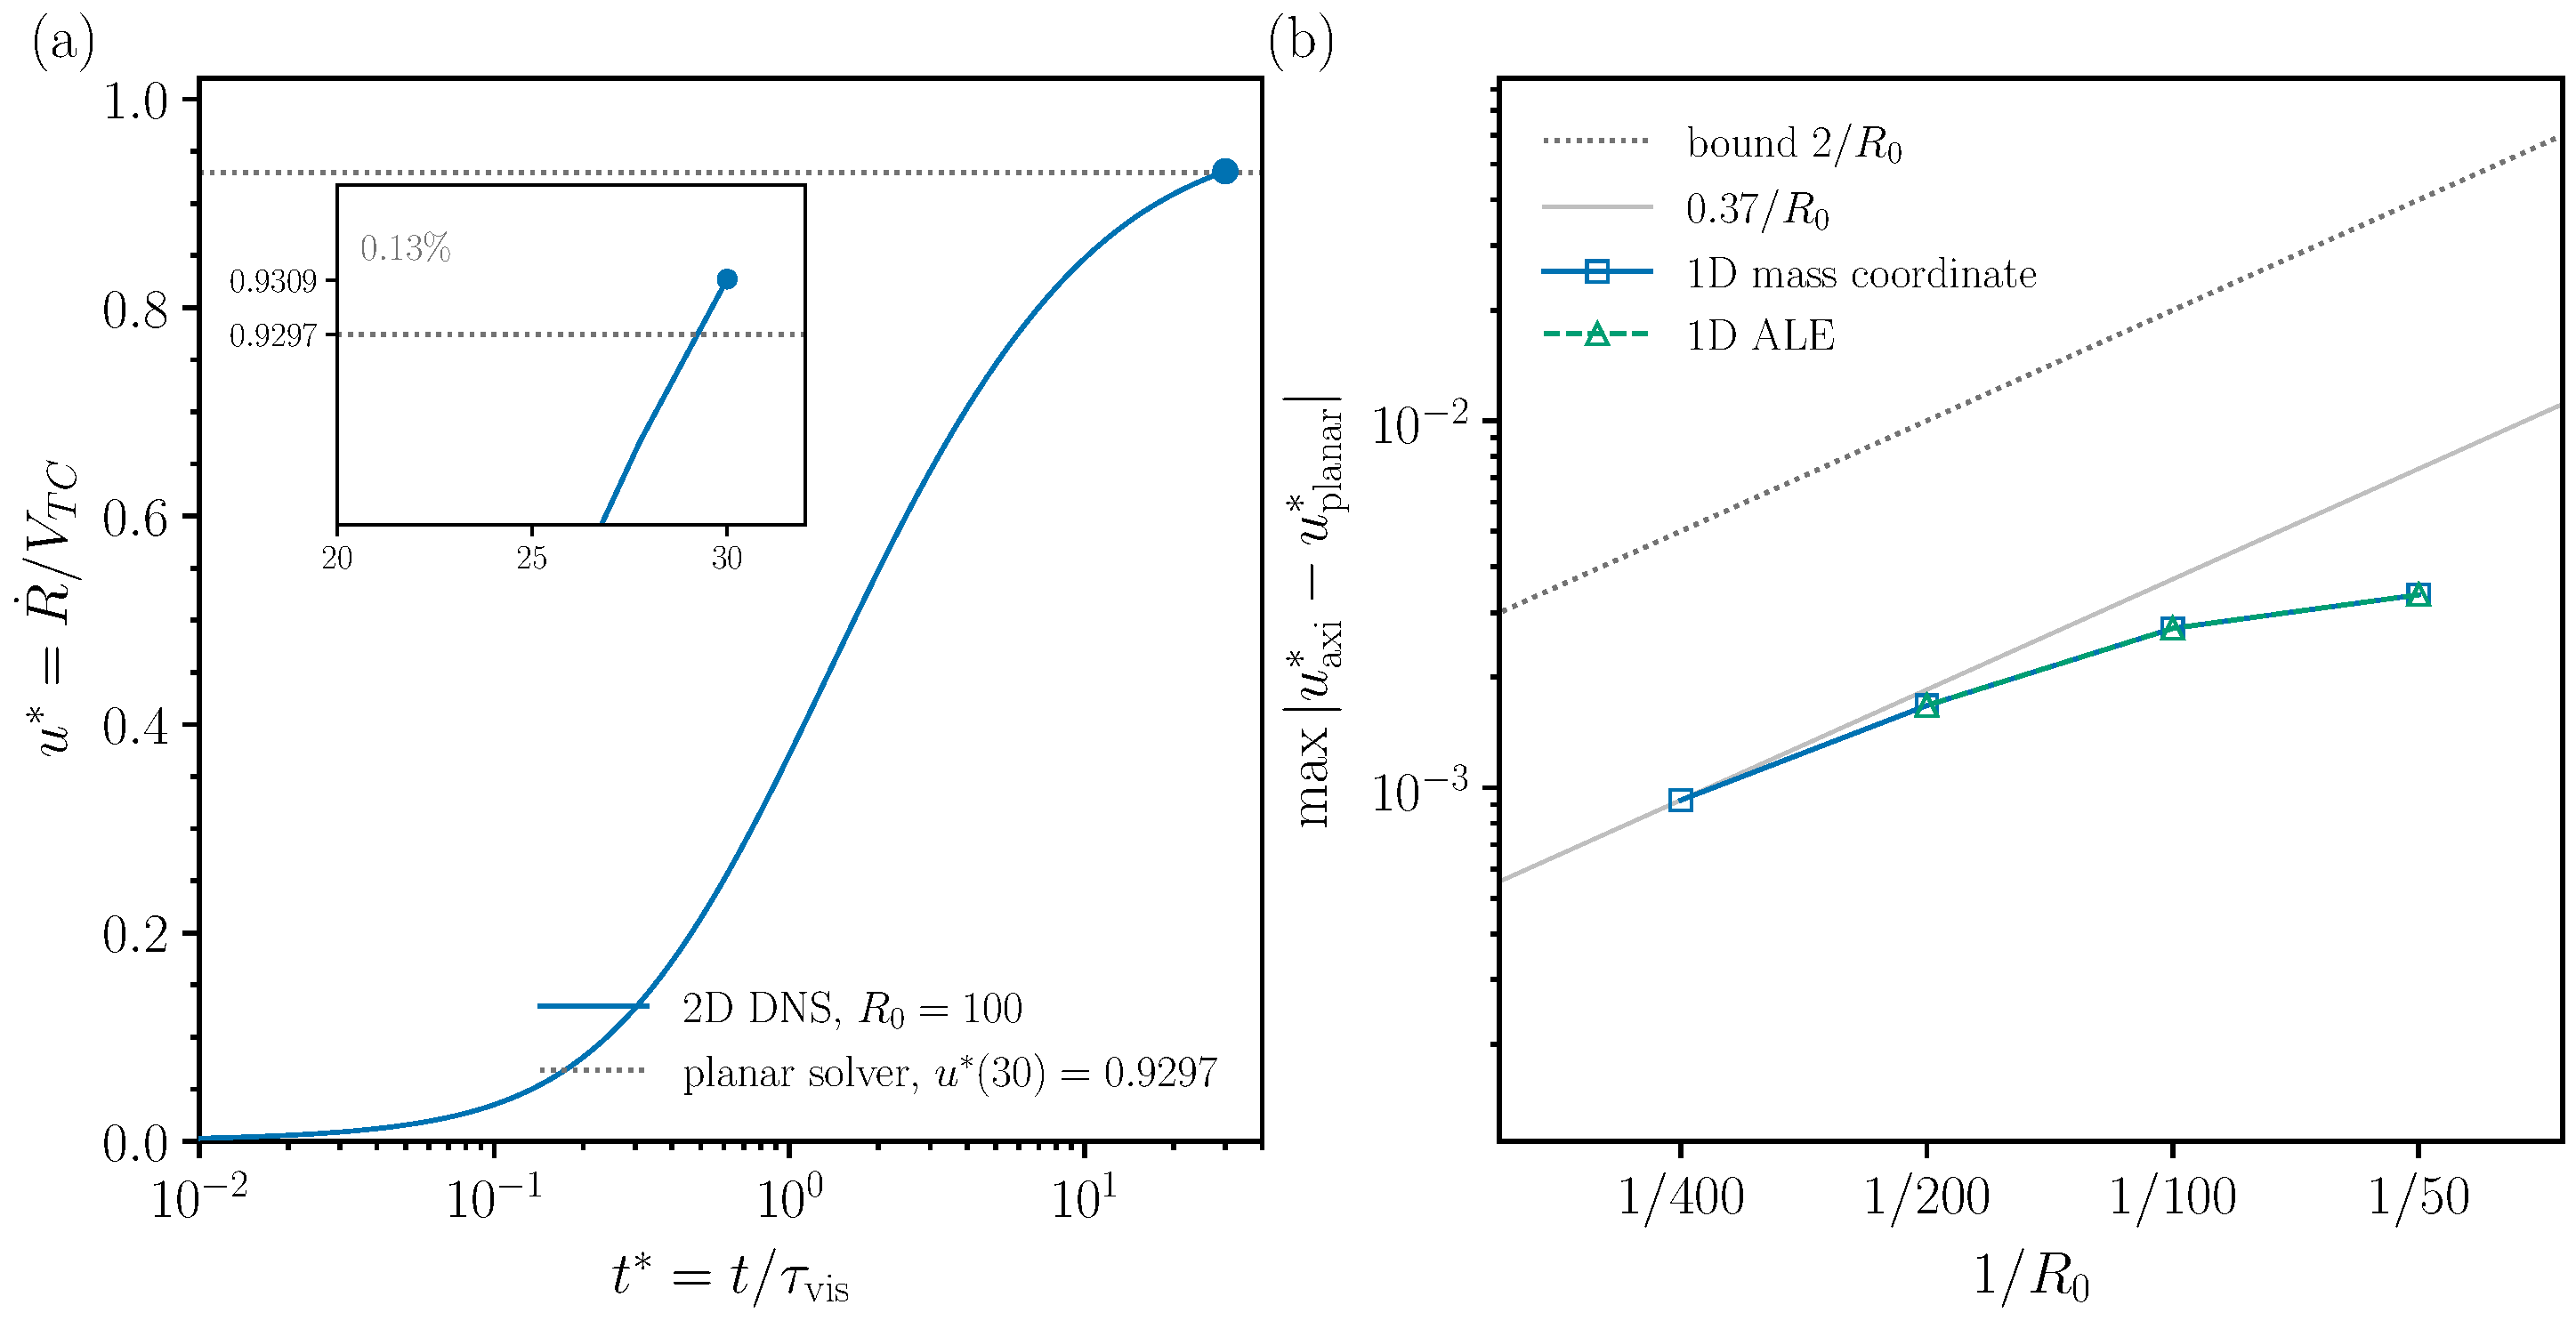
\includegraphics[width=\textwidth]{figures/fig2_planar_reduction.pdf}
  \caption{The planar-reduction gate. (a) The direct solver at $R_{0}=100$,
  $\Ohsb=0.5$, against the validated planar value $u^{*}(t^{*}=30)=0.9297$; the
  inset resolves the $0.13\%$ gap that the main axes cannot show. (b) The
  depth-averaged planar-limit ladder at $\Ohsb=1$: squares \MASS, triangles
  \ALE, dotted the $2/R_{0}$ admission bound, grey the line $0.37/R_{0}$. The
  two depth-averaged solvers are indistinguishable at this scale --- they agree
  to four significant figures at every rung --- so the two symbols overlie each
  other; that agreement is the cross-solver check of \S\ref{sec:verif-ale} seen
  from a second direction.}
  \label{fig:planar}
\end{figure}

\subsection{The direct solvers}
\label{sec:verif-lab}

\emph{Hoop-curvature discriminator.} A static quarter-disc droplet of radius
$a$ is solved to stationarity and its volume-averaged pressure compared with
Young--Laplace. The axisymmetric answer is $2\sigma/a$ and the planar answer
$\sigma/a$, so the factor of two is a clean discriminator that the azimuthal
curvature is genuinely active rather than the coordinate system merely being
labelled axisymmetric. Measured over a resolution ladder the exponent comes out
at $p = 1.9997$--$1.9999$ against $2$.

This check has a trap of its own, recorded because it produced a converged and
meaningless answer. Without mesh position degrees of freedom the free-surface
condition resolves to its static branch, and the kinematic multiplier then
enforces $\mathbf{u}\cdot\mathbf{n}=0$ as a rigid-wall reaction, absorbing the
entire surface-tension load itself and leaving the bulk pressure at solver
noise. The residual converges to machine precision in one Newton step; the
system is simply rank-deficient for the pressure. Adding the smoothed mesh
routes the multiplier into the mesh-position equation instead, which changes
which equation the multiplier feeds and not the physical answer.

\emph{Jacobian.} The analytic Jacobian agrees with a finite-difference Jacobian
over several steps of the real case at coarse resolution, with no aborts.

\emph{Volume.} Relative drift is $2.1\times10^{-9}$ over 200 steps with
remeshing suppressed, and about $2.6\times10^{-5}$ over a full remeshing run.
The difference is the interpolation error of the remesh operations, not
accumulation, and is discussed in \S\ref{sec:limits}.

\emph{Resolution ladders.} At $R_{0}=1$ the resolution knob was itself checked
before being used, because the total element count is insensitive to it on a
large domain and that insensitivity had been read as the knob doing nothing.
The minimum interface edge length at the tip tracks the requested resolution to
within $0.5\%$ of the ratio ($2.00$ for a factor-of-two change), and the near-tip
element count scales as the analytic grading law predicts; what goes flat is the
total count far from the tip, so counting elements over the whole annulus is
simply not a valid diagnostic here. On that verified ladder, halving the tip
edge length moves $R(t^{*}=50)$ by $5\times10^{-7}$ relative. Doubling the
output density --- which is what sets the timestep --- moves $R(50)$ by
$1.9\times10^{-6}$ and $\dot{R}(50)$ by $4.3\times10^{-4}$.

\emph{Window against wall.} The co-moving and laboratory solvers were run on the
same physical problem over an early window at resolution $0.06$, and their hole
radii agree to $|R_{\mathrm{com}}-R_{\mathrm{lab}}| \le 3.05\times10^{-5}$. The
co-moving solver's solved-unknown speed reads $U = 1.08498$ against the
laboratory solver's differenced $1.083$. The modified volume identity of
\S\ref{sec:comoving} holds to $7.2\times10^{-8}$ relative --- which is the
laboratory case's own volume drift on the same mesh, so the identity is
satisfied to the accuracy at which conservation itself holds, and the window
bookkeeping adds nothing measurable.
The long-window demonstration completed: with $L = 40$ the window carried the
tip to $R = 38.77$ at $t = 30$ ($u^{*} = 0.940$ and rising toward $\sqrt{2}$),
more than three times the radius at which the laboratory annulus used in
\S\ref{sec:validation} exhausts its domain, at a per-step cost that does not
grow with $R$ --- the structural property the window formulation exists to
provide. The modified volume identity held to $3.5\times10^{-7}$ relative over
the whole run, and a second run at $1.6\times$ coarser resolution reproduced
$R(30)$ to $0.13\%$. The $L$-convergence ladder ($L = 20/40/80$) that would
establish window-length independence is deliberately left to the follow-up
campaign; $L = 40$ is asserted from the planar experience, not measured.

\section{Validation}
\label{sec:validation}

Three external comparisons, one end-to-end run each.

\subsection{Reduction to the planar problem}

At $R_{0}=100$ and $\Ohsb=0.5$ the direct axisymmetric solver returns
$u^{*}(t^{*}=30) = 0.9309$ against the validated planar value $0.9297$, a
difference of $0.13\%$ (figure~\ref{fig:planar}(a)). The expected residual
curvature effect at this radius is $O(h_{0}/R)\approx 1\%$ at the start and
smaller as the hole grows, so a tenth of a percent is the right order and the
right sign. This is the direct-solver counterpart of the depth-averaged gate in
\S\ref{sec:planarlimit}, and it exercises a completely different code path: a
free surface with both curvatures, a moving mesh, remeshing, and the Newton
tolerance law of \S\ref{sec:trap-newton}.

\subsection{Against a volume-of-fluid campaign}
\label{sec:basilisk}

At coded $\Ohsb = 0.7071$ and $R_{0}=1$ the initial condition matches that of
the 2024 volume-of-fluid campaign exactly, so no parameter matching is required.
Over the record the two agree to $1.6\%$ in the hole radius and $1.8\%$ in the
tip speed. The discrepancy is systematic rather than scattered, and it is quoted
at face value: the reference's own resolution study is not recorded, so it
cannot be attributed to either side. Appendix~\ref{sec:audits} reports a
source-level audit whose purpose was to determine whether the difference could
be a missing term on the finite-element side. It is not: every axisymmetric term
the volume-of-fluid code adds by hand corresponds one-to-one with a term the
finite-element tensor layer generates automatically, and the metric factors are
exact. The ranked candidates that remain are all on the volume-of-fluid side.
\todo{the fresh Newtonian axisymmetric rerun of the reference code, which will
either reproduce the 2024 curves or localise the offset in the campaign rather
than the method}

At $R_{0}=1$ the direct solver shows a mesh-independent feature that the
depth-averaged model cannot represent at all. The tip does not open
monotonically: the hole radius \emph{closes} by $0.49\%$, reaching its minimum
near $t = 0.15$, before turning around and growing smoothly with $\dot{R}$
climbing towards $\Vtc$. The shape is identical at two resolutions differing by
a factor of four in near-tip element count, and it is the interface--symmetry
corner node itself that recedes. The mechanism is the one the tip correction
\eqref{eq:tipcorr} describes: at $R\sim h_{\mathrm{tip}}\sim1$ the toroidal term
is $O(1)$ against the leading $-2$, the net driving force is genuinely weak, and
at low Ohnesorge number an impulsively started flow can transiently go the
other way. The proximity to the Taylor \& Michael closing threshold
\cite{taylor1973} is not incidental. A quasi-static massless-cap closure, with
either constant, has no way to encode ``weak enough to be beaten by inertia for
a while'' and so cannot produce this at all.

\subsection{The depth-averaged model against the direct solution}
\label{sec:bracket}

The comparison at $R_{0}=1$ requires care with the initial condition. The direct
solver's cap of radius $1/2$ carries volume that the clean-hole depth-averaged
initial condition does not, so the reduced model is started at the
volume-matched radius
%
\begin{equation}
  R_{\mathrm{eq}}^{2} = r_{s}^{2} - \frac{\pi a r_{s}}{2} + \frac{2a^{2}}{3},
  \qquad r_{s} = R_{0}+a, \quad a = \tfrac{1}{2},
  \label{eq:req}
\end{equation}
%
giving $R_{\mathrm{eq}} = 1.1129$ for $R_{0}=1$. The quantity compared is
$\dot{R}$ and not $R$: the depth-averaged tip is the matched edge of an
asymptotic construction while the direct hole radius is the innermost interface
point, and the offset between them is an irreducible $O(h/2)$.

At $\Ohsb = 0.7071$ and $t^{*} = 100$,

\begin{center}
\begin{tabular}{@{}lc@{}}
\toprule
 & $u^{*}(t^{*}=100)$ \\
\midrule
direct solver (\LAB) & $0.9613$ \\
\ALE, default closure $N_{rr}(R)=-2$ & $0.9966$ \\
\ALE, with toroidal correction \eqref{eq:tipcorr} & $0.8976$ \\
\bottomrule
\end{tabular}
\end{center}

The two closures bracket the direct solution, from $+3.7\%$ above and $-6.6\%$
below (figure~\ref{fig:bracket}). Neither is right, and that is the result: at
$R_{0}\sim1$ the azimuthal curvature contributes an $O(1)$ fraction of the edge
force, so the leading-order closure omits a term of its own order, while the
first correction \eqref{eq:tipcorr} overshoots it. The discrepancy is located in
the edge condition and not in the bulk operators, which is exactly what
bracketing establishes and what a single closure could not. The sign of the
default closure's error is also informative: its overshoot is the same
planar-style bias the reduced model shows against the direct solution in the
planar geometry, so it is inherited rather than new.

\begin{figure}[htbp]
  \centering
  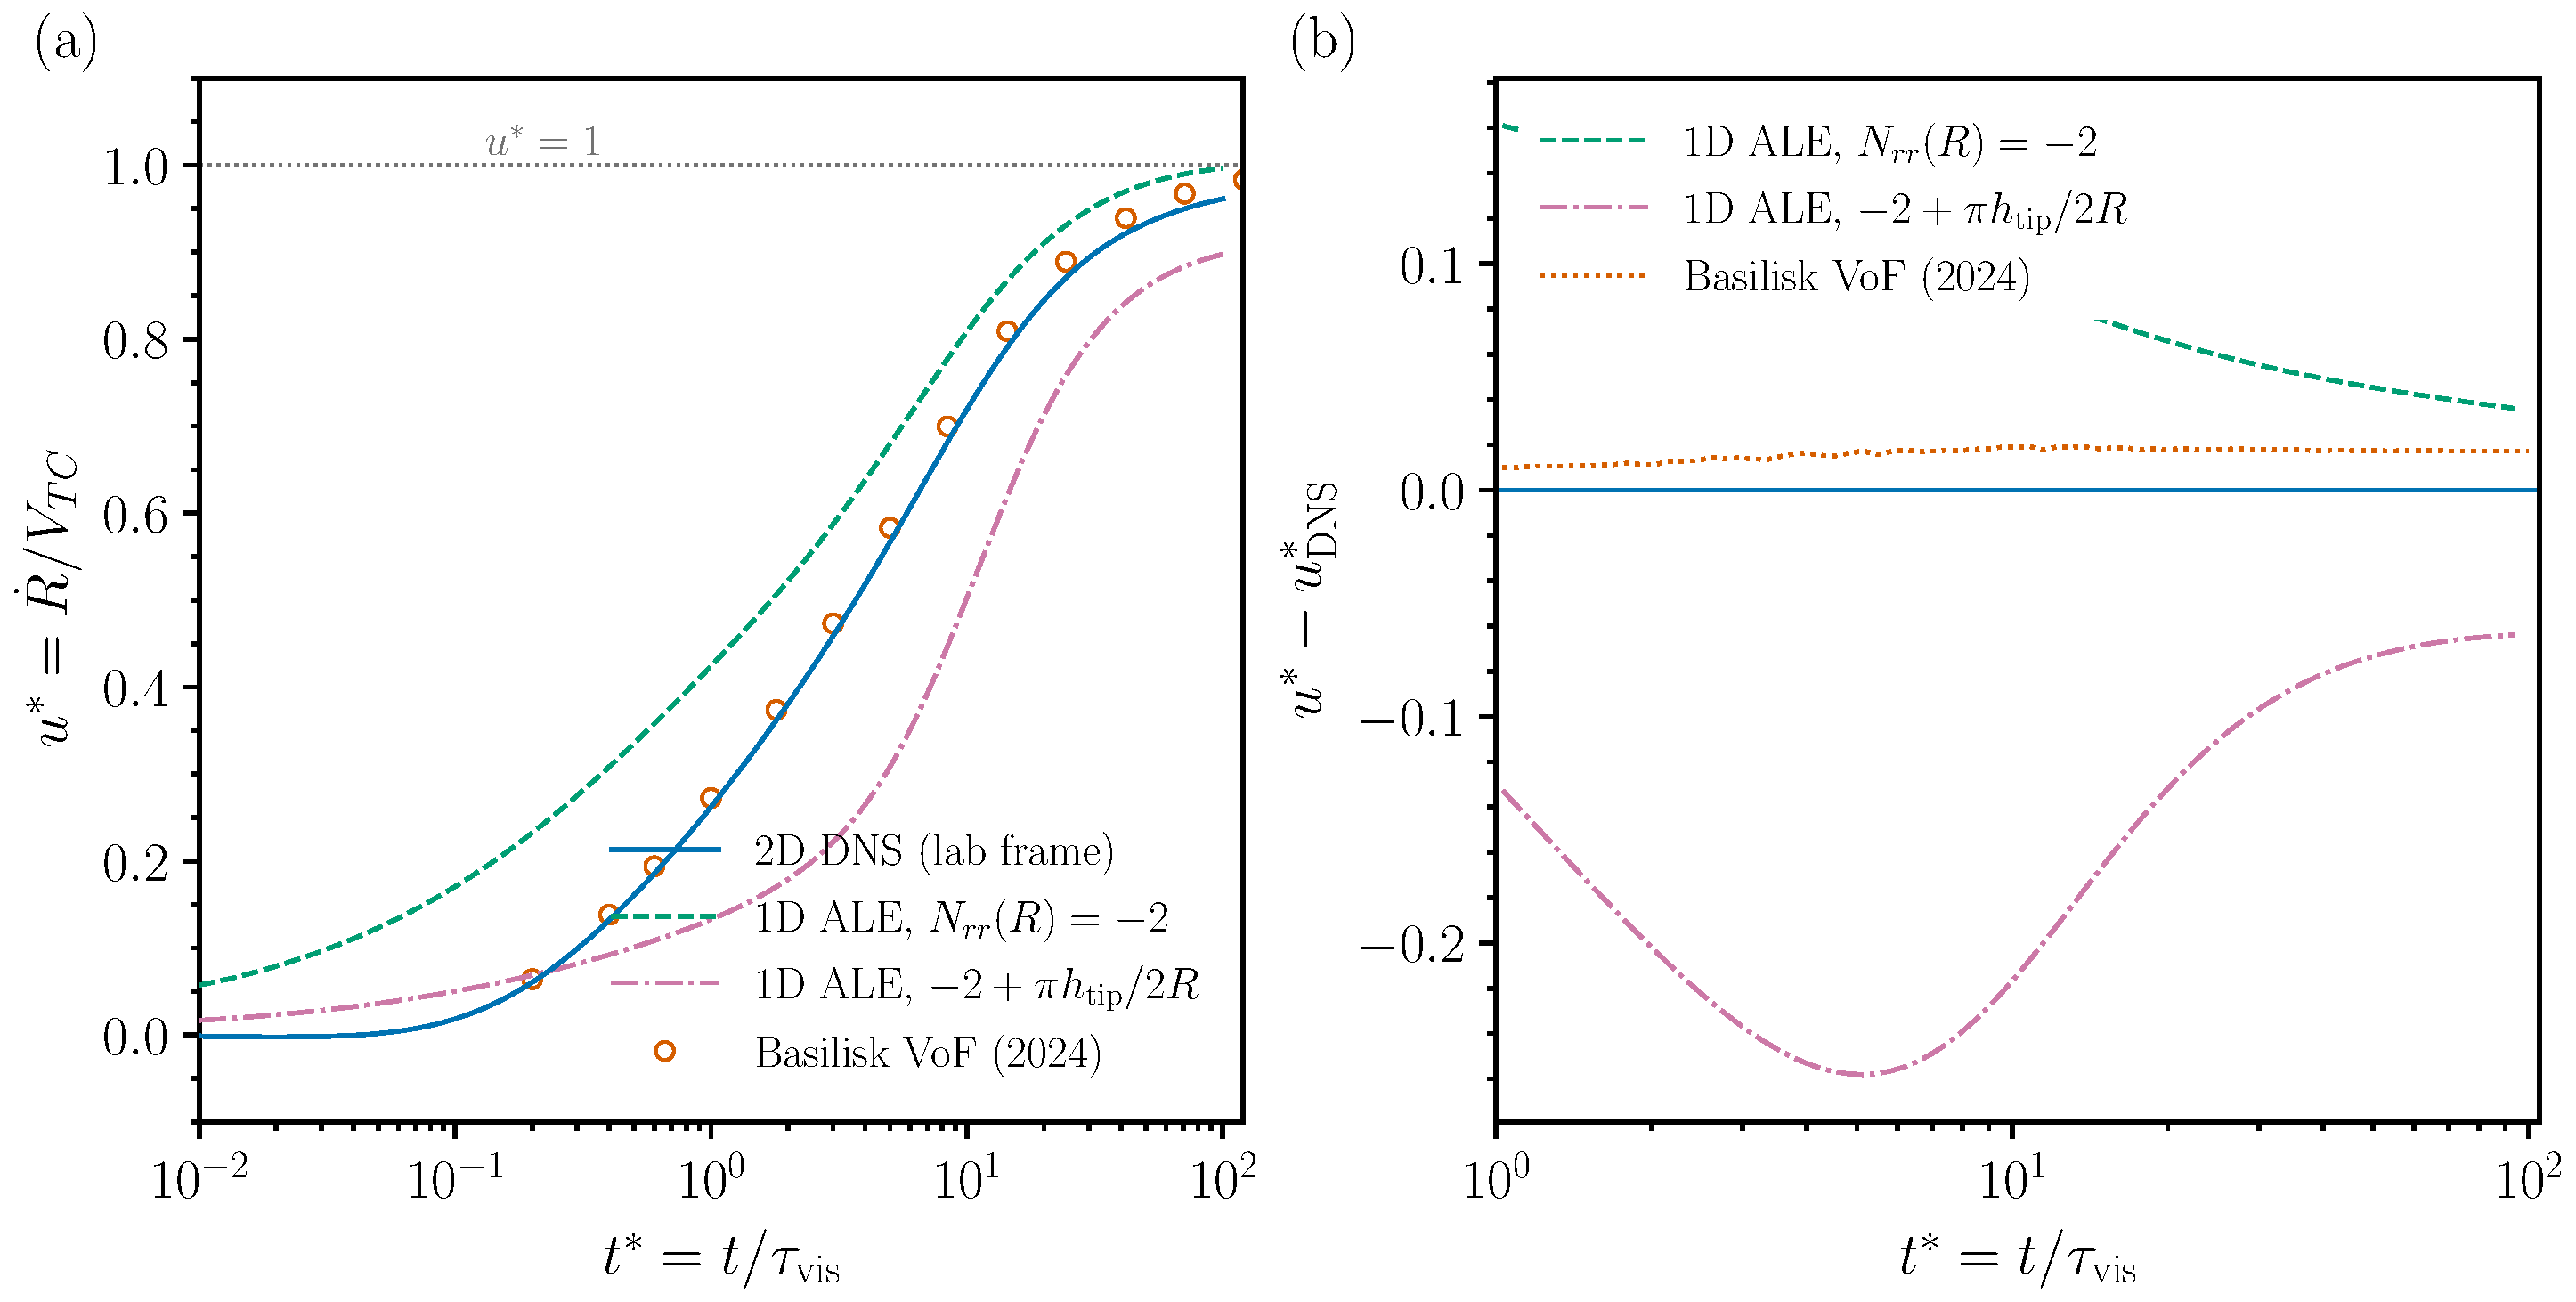
\includegraphics[width=\textwidth]{figures/fig1_closure_bracket.pdf}
  \caption{The two tip closures bracket the direct solution at $\Ohsb=0.7071$,
  $R_{0}=1$. (a) Retraction speed: solid, direct solver in the laboratory
  frame; dashed, \ALE\ with the default closure $N_{rr}(R)=-2$; dash-dot, \ALE\
  with the toroidal correction \eqref{eq:tipcorr}; circles, the 2024
  volume-of-fluid campaign. The depth-averaged runs start at the volume-matched
  radius \eqref{eq:req}. The direct record is genuinely negative over the first
  $\sim0.2$ viscous times --- the tip recedes before it opens
  (\S\ref{sec:basilisk}) --- and is drawn on linear ordinates so that it is
  visible rather than eaten by a logarithmic axis. (b) Departure from the direct
  solution, on the direct solver's own abscissa; the other three records are
  interpolated onto it, which is safe here because all four are smooth and
  monotone over the window shown. The two depth-averaged curves lie on opposite
  sides of zero over the whole record.}
  \label{fig:bracket}
\end{figure}

The mass-coordinate solver was run in the same configuration as a
cross-check. Its first attempt terminated in the Newton floor of
\S\ref{sec:trap-newton} --- the observation that motivated porting the
$\varepsilon\,r_{\max}^{2}/\Delta t$ tolerance rule to that solver --- and the
repaired rerun advanced well past the original failure times ($t^{*} = 73$ and
$88$ of $100$) but was stopped short of completion as outside this strand's
scope. It is therefore omitted from figure~\ref{fig:bracket} rather than
plotted short. The two solvers agree to $7.3\times10^{-6}$ over the range where
both are available (\S\ref{sec:verif-ale}), so nothing in the conclusion turns
on it.

Two of Savva \& Bush's axisymmetric curves were digitised with the same
calibrated workflow as the planar figures (\texttt{validation/data/}, with
per-figure calibration overlays): their figure~16 inset curve~C
($\mathrm{Oh}_{\rm SB} = 1$, $R_{0} = 50H$ --- at this Ohnesorge number their
viscous and inertial clocks coincide, so the comparison is
convention-proof) and figure~10 curve~G ($\mathrm{Oh}_{\rm SB} = 10$,
$R_{0} = 50H$, viscous clock). Against the mass-coordinate solver at matched
$R_{0}$: at $\mathrm{Oh}_{\rm SB} = 1$ over $t^{*} \in [2, 10]$ the default
closure agrees to $1.9\%$ rms ($u^{*}(10) = 0.9133$ against their $0.8985$),
and the toroidal tip correction \emph{improves} this to $1.3\%$ rms --- their
model resolves the smoothed rim cap with full capillarity, which is exactly
the physics the correction reinstates at leading order. At
$\mathrm{Oh}_{\rm SB} = 10$ over $t^{*} \in [2, 34.5]$ the agreement is
$3.5\%$ rms with the deviation concentrated in the early transient
(where their published sensitivity to the initial tip-smoothing parameter
$\alpha$ is strongest, their figure~14) and narrowing to $1.8\%$ by
$t^{*} = 34.5$. Digitisation accuracy is $0.15$--$0.3\%$ of full scale. A
third digitised curve (their figure~16 main panel, curve~D) is retained in
the data directory but excluded here: its time-axis normalisation in the
moderate-Oh section could not be established beyond doubt, and a comparison
built on a guessed clock would be worse than none. The self-similar collapse
at matched $\Ohsb\,h_{0}/R_{0}$ remains the natural test to build on these
curves.

\section{Four numerical traps}
\label{sec:traps}

Each of these cost real time, and three of them present as something other than
what they are. They are recorded with the evidence that discriminated the cause,
because in every case the plausible first diagnosis was wrong.

\subsection{The Newton absolute-tolerance floor}
\label{sec:trap-newton}

\emph{Symptom.} A run at large radius aborts inside its first output interval
with residuals oscillating at $O(0.1)$ and the timestep controller halving until
it refuses to go further. The oscillation looks structural and looks independent
of the timestep, and is neither.

\emph{Cause.} The solver's convergence test is an absolute bound on the
max-norm of the residual vector, and the axisymmetric coordinate system
multiplies every residual entry by $2\pi r$. The residual magnitude of the same
physical imbalance therefore grows linearly with the hole radius. A direct solve
cannot drive a residual below roughly $\varepsilon\|J\|\,\|u\|$; here $\|u\|$ is
dominated by mesh-position unknowns, which are absolute radii $\sim R$, and
$\|J\|$ by the mass rows, which carry the measure weight $\sim R$ divided by the
timestep. Hence a floor $\sim \varepsilon R^{2}/\Delta t$. Every rejected step
halves $\Delta t$, which \emph{raises} the floor, so the cascade is
self-reinforcing and the $O(0.1)$ oscillation is its tail rather than its cause.

\emph{Discriminating evidence.} A one-variable-at-a-time scan in $R_{0}$ at
identical mesh, unknown count and timestep gives initial residuals exactly
linear in $R_{0}$ and final residuals $2.8\times10^{-11}$, $5.3\times10^{-10}$,
$7.6\times10^{-9}$ and $3.7$--$5.2\times10^{-8}$ at $R_{0}=1$, $10$, $30$ and
$100$; only the last never stops, so only the last measures a floor rather than
bounding it. A smooth onset that tracks the coordinate offset is a scaling, not
a defect that switches on. Independently, a timestep scan at fixed $R_{0}=100$
gives floors from $9.2\times10^{-10}$ at $\Delta t = 6.8\times10^{-4}$ to
$2.0\times10^{-6}$ at $\Delta t = 3.4\times10^{-7}$, tracking
$\varepsilon R^{2}/\Delta t$ to within a factor of about five throughout. What
it is \emph{not} was checked in each case: not a residual or Jacobian error (the
finite-difference Jacobian is clean at $R_{0}=100$, and the identical
configuration converges to $6.1\times10^{-10}$ at a larger timestep), not the
graded mesh (the failure reproduces on a uniform one), not the Newton budget
(the residual sits at the same value for a further thirty-one iterations, and a
line search does not move it), and not the time-integrator start-up.

\emph{Remedy.} Retune the tolerance per timestep as
$\max(\varepsilon_{0}, \, s\,\varepsilon R^{2}/\Delta t)$ with a safety factor
$s$, which holds roughly a thirtyfold margin over the measured floor uniformly
in $\Delta t$. A fixed tolerance is a lottery, because the last sub-step of an
output interval is a leftover sliver whose floor may be orders of magnitude
above the interval's. Rescaling the test space by $1/R$ instead would move one
of the two factors into the residual and leave the Newton step identical; it
would not touch the $1/\Delta t$ factor, which is the one that kills runs. In
the window formulation the scale is read live from the global position unknown
rather than from the initial radius, since $R$ is no longer approximately
constant.

This trap appeared three times in this strand, with three different scales:
$R_{0}^{2}$ in the laboratory solver, $(X+L)^{2}$ in the window solver, and
$R_{0}^{2}+2M$ in the mass-coordinate solver, where the domain is a mass and the
largest radius is $\sqrt{R_{0}^{2}+2M}$. The last of these is why the
mass-coordinate legs of \S\ref{sec:bracket} are short: at the comparison's
domain size the floor is three orders of magnitude above what the check suite's
shorter horizons ever see. The depth-averaged ALE solver meets the same
mechanism in a milder form --- Newton lands on a genuine fixed point, or a
two-cycle between two bit-identical values, at a few times $10^{-8}$ and errors
out only because that is just above tolerance --- and is cured by a fixed looser
absolute tolerance, still nine orders tighter than the velocity scale of the
physics, verified over $R_{0}\in\{5,200,1000\}$ and three decades of starting
step.

The underlying absolute test is inherited from the upstream library
\cite{heil2006}; no relative criterion exists there either, so the per-step
retune is the correct local remedy and a relative-tolerance option is upstream
work.

\subsection{A double Lagrange multiplier at the outflow corner}
\label{sec:trap-corner}

\emph{Symptom.} In the window formulation the linear solver reports a backward
error of order $10^{47}$, the first Newton step returns a non-finite value, and
every timestep is rejected until the controller refuses to reduce further. That
last part reads exactly like the cascade of \S\ref{sec:trap-newton} and is a
completely different failure. A finite-difference Jacobian check does not catch
it: the assembled Jacobian is correct, and it is the system that is
rank-deficient.

\emph{Cause.} At the corner where the outflow boundary meets the free surface,
the axial mesh coordinate is pinned but the radial one is a free unknown, and
two Lagrange multipliers act on that one unknown --- the free surface's
kinematic multiplier and the multiplier enforcing the window's far edge. Two
constraints on one unknown is a null space. The laboratory case never sees it,
because an ordinary Dirichlet condition removes the position unknowns and the
framework then disposes of the orphaned kinematic multiplier itself.

\emph{Discriminating evidence.} The singular values of the assembled Jacobian,
smallest first, are $4.8\times10^{-13}$, $2.3\times10^{-12}$,
$4.6\times10^{-4}$ as written; pinning the corner multiplier removes the first
and leaves $2.3\times10^{-12}$, $4.6\times10^{-4}$; the laboratory case on the
same mesh gives $2.3\times10^{-12}$, $4.7\times10^{-4}$. The largest singular
value is $5.3\times10^{3}$, and there are no zero rows or columns, so the
deficiency is structural rather than a missing entry. The offending mode is
entirely in the kinematic multiplier, dominated by a single node with an
exponentially decaying tail along the interface --- the signature of one
redundant constraint, not of a physical soft mode. The mode that survives is not
introduced here at all: the laboratory case carries the identical mode at the
same magnitude. Pinning the corner multiplier therefore restores the working
case's conditioning exactly, and nothing more.

Two further points of the same formulation are worth recording because each was
initially written the natural way and was wrong. The tip-pinning constraint must
be written in residual form as $\texttt{mesh\_x} - X$ rather than as
$\texttt{mesh\_x}$: the tip sits at $r\sim R_{0}>0$, so under the $2\pi r$ point
measure the constraint $2\pi r_{\mathrm{tip}}\,\texttt{mesh\_x}_{\mathrm{tip}} =
0$ is a double root whose derivative vanishes at the solution, giving a singular
Jacobian row, whereas $\texttt{mesh\_x} - X$ has derivative $-1$ identically.
And that pin must be evaluated in a Cartesian measure: it is a geometric
statement that a node sits at a radius, not an integral of anything, and the
$2\pi R(t)$ factor an axisymmetric measure would attach to it grows without
bound over a long window run.

\subsection{An argument-parser prefix collision}
\label{sec:trap-argv}

The framework parses the real command line at problem initialisation, with
prefix matching active, and one of its own flags is \texttt{--outdir}. A
script's own \texttt{--out} option is therefore accepted as that flag and
silently overrides every per-case output directory in the process. There is no
error and no warning; runs simply write somewhere else. The remedy in the
drivers is to suppress command-line parsing outright; in the check scripts,
which also invoke the planar reference through a driver that does not suppress
it, the argument vector is emptied before the first solver is constructed.
This is recorded because the symptom --- output appearing in one directory when
several were requested --- reads as a bug in the script's own path handling.

\subsection{An unbounded domain estimate}
\label{sec:trap-domain}

The small-hole exponential law $R = R_{0}\exp(t^{*}/2)$ is an \emph{early-time}
statement: it holds only while the edge speed $R/(2\tau_{\mathrm{vis}})$ is
below $\Vtc$, that is until $R$ reaches the crossover radius $\sqrt{2}\mu$, past
which the edge cannot outrun the Taylor--Culick speed. Sizing a domain from the
raw exponential at a large end time therefore requests an astronomically long
mesh --- of order $10^{21}$ at $t^{*}=100$ --- and the resulting mesh
coordinates blow the first Newton solve up to residuals of order $10^{34}$,
which is how the bound was found. The driver now computes both the exponential
estimate, capped at the crossover radius, and the linear estimate $\Vtc t$, and
takes the larger: no single formula covers the whole range of $R_{0}^{*}$. The
estimate is a starting point and not a promise, and every output leg checks the
far-field drift.

A related sizing point is worth stating because the planar rule looks
transferable and is not. In the mass coordinate the domain is
$M = \int_{R}^{r_{\max}} r h\,\mathrm{d}r$, which for an undisturbed film is
$(r_{\max}^{2}-R_{0}^{2})/2$ --- quadratic in the radial extent. Reusing the
planar expression, which returns a length, sizes the domain by a factor of order
$r_{\max}$ too small.

\section{Limitations, and what would remove them}
\label{sec:limits}

\emph{Window-length convergence is not established.} The window formulation has
been verified against the laboratory solver over an early window
(\S\ref{sec:verif-lab}), which tests that the two agree where both are valid. It
has not been run long enough for the semi-infinite behaviour it exists to
capture, and the window length $L$ has not been varied. Until an $L$-ladder
exists, a long window run reports a length as much as a physics.

\emph{The smoke ladder does not cover large $R_{0}$.} The quick physics probe
runs at $R_{0}=1$; the planar-reduction case at $R_{0}=100$ is a multi-hour
comparison and is deliberately not a smoke test. The consequence is that the
Newton tolerance law of \S\ref{sec:trap-newton} is exercised by the campaign
rather than by the fast checks, and its scale is set from the \emph{initial}
radius rather than the live one. Over the runs reported here $R$ grows by about
$15\%$, so the distinction does not bite; a campaign in which $R$ grows by an
order of magnitude from a large $R_{0}$ should re-measure rather than assume.

\emph{Remeshing costs volume conservation four orders of magnitude.} Drift is
$2.1\times10^{-9}$ over 200 steps without remeshing and about
$2.6\times10^{-5}$ over a full run with it. The difference is interpolation at
the remesh, not accumulation between them, so it is bounded by the number of
remeshes rather than by the run length --- but it does set the floor on what the
volume identity can certify, and it is the reason the window's modified identity
is quoted as matching the laboratory case's own drift rather than as being
exact.

\emph{The tip closure is bracketed, not determined.} \S\ref{sec:bracket} shows
that the leading-order closure and its first geometric correction lie either
side of the direct solution at $R_{0}\sim1$. That localises the error and does
not fix it. Two routes are open: a systematic $O(h/R)$ matched-asymptotic
treatment of the toroidal rim, which would replace \eqref{eq:tipcorr} with a
derived rather than an estimated coefficient; and an inertial cap, which is what
the transient reversal of \S\ref{sec:basilisk} indicates is missing, since a
quasi-static massless cap cannot produce it at any coefficient. The second is
the more interesting because it is a statement about the model rather than about
its constant.

\emph{The comparison set is thin by design.} One run per question, no sweep in
$\Ohsb$ or $R_{0}$, and no digitised axisymmetric literature curves. The
verification evidence of \S\ref{sec:verification} is meant to carry the weight
that a sweep would otherwise carry, and it is worth being explicit that it
cannot carry all of it: internal consistency at high precision is not external
agreement.

\appendix

\section{Two source-level audits}
\label{sec:audits}

Both were run after the validation gates of \S\ref{sec:validation} had passed,
to answer a question the gates raise but cannot settle: whether the residual
disagreement with the volume-of-fluid reference could be a term missing on the
finite-element side.

\emph{Against the volume-of-fluid code's axisymmetric module.} Every
axisymmetric term that code adds by hand --- the hoop-viscosity patch in its
viscous solver, the three separate azimuthal-curvature additions in its
curvature routine, and, for the viscoelastic extension, a bespoke hoop-stress
field with its own momentum forcing --- corresponds one-to-one with a term the
finite-element tensor layer produces automatically: the $u_{r}/r$ entry of the
velocity gradient, the $(T_{rr}-T_{\theta\theta})/r$ entry of the tensor
divergence, and the surface divergence. No physics is missing on the
finite-element side, and the metric factors themselves are exact and are ruled
out as the source of the $1.6$--$1.8\%$ offset. The remaining candidates, ranked
and all on the volume-of-fluid side, are height-function curvature noise
together with the explicit floor that method places on the azimuthal curvature;
the hoop viscous term being an acknowledged after-the-fact patch; adaptive
coarse/fine transitions at the rim; and the resolved ambient phase that a
single-phase formulation excludes. A useful corollary for the viscoelastic
extension: the polymeric hoop stress will arrive through the tensor divergence
with no bespoke module.

\emph{Against the underlying library's hand-written axisymmetric elements.} The
residuals generated for \LAB\ are term-for-term identical to the library's
axisymmetric Navier--Stokes element --- momentum including the $u_{r}/r^{2}$
hoop viscous and $p\psi/r$ hoop pressure terms, the continuity radius factors,
the ALE corrections and the stress-divergence form --- and to its axisymmetric
interface element, including the azimuthal-curvature injection in the
surface-divergence capillary term, up to a global factor of $2\pi$ and a global
sign \cite{heil2006}. The one omitted end-of-interface co-normal term lands
entirely in pinned equations at both ends, so it is discarded correctly rather
than lost. This audit is also where the absolute Newton tolerance of
\S\ref{sec:trap-newton} was traced upstream.

\begingroup
\let\oldthebibliography\thebibliography
\renewcommand{\thebibliography}[1]{%
  \oldthebibliography{#1}%
  \setlength{\itemsep}{0pt plus 0.2ex}%
  \setlength{\parskip}{0pt}}
\bibliographystyle{unsrt}
\bibliography{axi-validation}
\endgroup

\end{document}
